% Oklahoma application section — edit freely. Regenerate table numbers and plots with:
%   Rscript inst/oklahoma/paper/oklahoma_paper_assets.R
%
% From the repository root (or adjust paths / \graphicspath):
%   % Oklahoma application section — edit freely. Regenerate table numbers and plots with:
%   Rscript inst/oklahoma/paper/oklahoma_paper_assets.R
%
% From the repository root (or adjust paths / \graphicspath):
%   % Oklahoma application section — edit freely. Regenerate table numbers and plots with:
%   Rscript inst/oklahoma/paper/oklahoma_paper_assets.R
%
% From the repository root (or adjust paths / \graphicspath):
%   % Oklahoma application section — edit freely. Regenerate table numbers and plots with:
%   Rscript inst/oklahoma/paper/oklahoma_paper_assets.R
%
% From the repository root (or adjust paths / \graphicspath):
%   \input{inst/oklahoma/paper/oklahoma_application_section}
% Preamble: \usepackage{booktabs}

\section{Seismic Activity in Oklahoma}\label{sec:application}

A sharp rise in seismicity in the US state of Oklahoma was observed after 2008. Existing research \cite{Keranen2014,WeingartenEtAl2015} attributes this increase primarily to high-volume wastewater (produced-water) disposal, especially disposal into the deep Arbuckle rock formations near basement-connected faults, rather than to hydraulic fracturing. Subsequent analyses \citep{WalshZoback2015} showed that earthquake activity clustered near large volume disposal wells and closely tracked rapid increases in disposal volumes in central Oklahoma . Later work refined the mechanism, emphasizing injection depth relative to crystalline basement and delayed pressure diffusion, which help explain both the regional spread of seismicity and the lagged decline in earthquake rates after disposal volumes were reduced \cite{LangenbruchZoback2016,Hincks2018}. Although Oklahoma has also experienced earthquakes directly associated with hydraulic-fracturing stages, that literature generally treats them as a distinct process and a smaller contributor to the statewide surge in seismicity during the 2010s \cite{RubinsteinMahani2015,SkoumalEtAl2018}.

On 18 March 2015 the Oklahoma Corporation Commission (OCC) issued a directive requiring disposal well operators within a designated Area of Interest (AOI) in central Oklahoma to reduce wastewater disposal volumes \cite{wertz2015regulators}. The AOI is a seismicly active area, where the Arbuckle rock formation is well suited to absorbing liquid. While a decline in seismicity is readily observed after the directive, estimating the actual causal effect of the policy is challenging due to temporal carry over, spatial spillover and non random treatment assignment. We target a DTAITE estimate where the comparison is control everywhere in Oklahoma vs the actual treatment regime, thus we will estimate the expected number of Earthquakes the policy prevented.

We restrict to earthquakes of at least magnitude 2.5 and consider bivariate epidemic-type aftershock sequence (ETAS) models \cite{ogata} for latent control and treated components with a shared triggering kernel and KDE-driven inhomogeneous background \cite{nandan2017objective}. We use the fist half of the pre treatment data to estimate the background rate and proceed with our SEM approach comparing it to the naive approach setting labels equal to the location treatment status.

Our chosen estimand of interest is the 100 day DTAITE, where the two treatment regimes are control everywhere, i.e. no directive was made and the actual observed treatment regime, denoted $\hat\Delta_{\mathrm{AoI}}=E[N(\mathrm{control\ everywhere})]-E[N(\mathrm{actual\ regime})]$. Table \ref{tab:ok_counts} shows the differences in expected counts for the ETAS model with parameters estimated with naive labelling and our SEM method.

\input{inst/oklahoma/paper/generated/tab_ok_counts}

Figure \ref{fig:ok-ef-bootstrap-hist} shows the distributions of a parametric bootstrapped DTAITE estimands using de-biased bootstrap replicates \cite{efron_boot}, there is limited overlap between the distributions suggesting a real difference.

\begin{figure}[htbp]
\centering
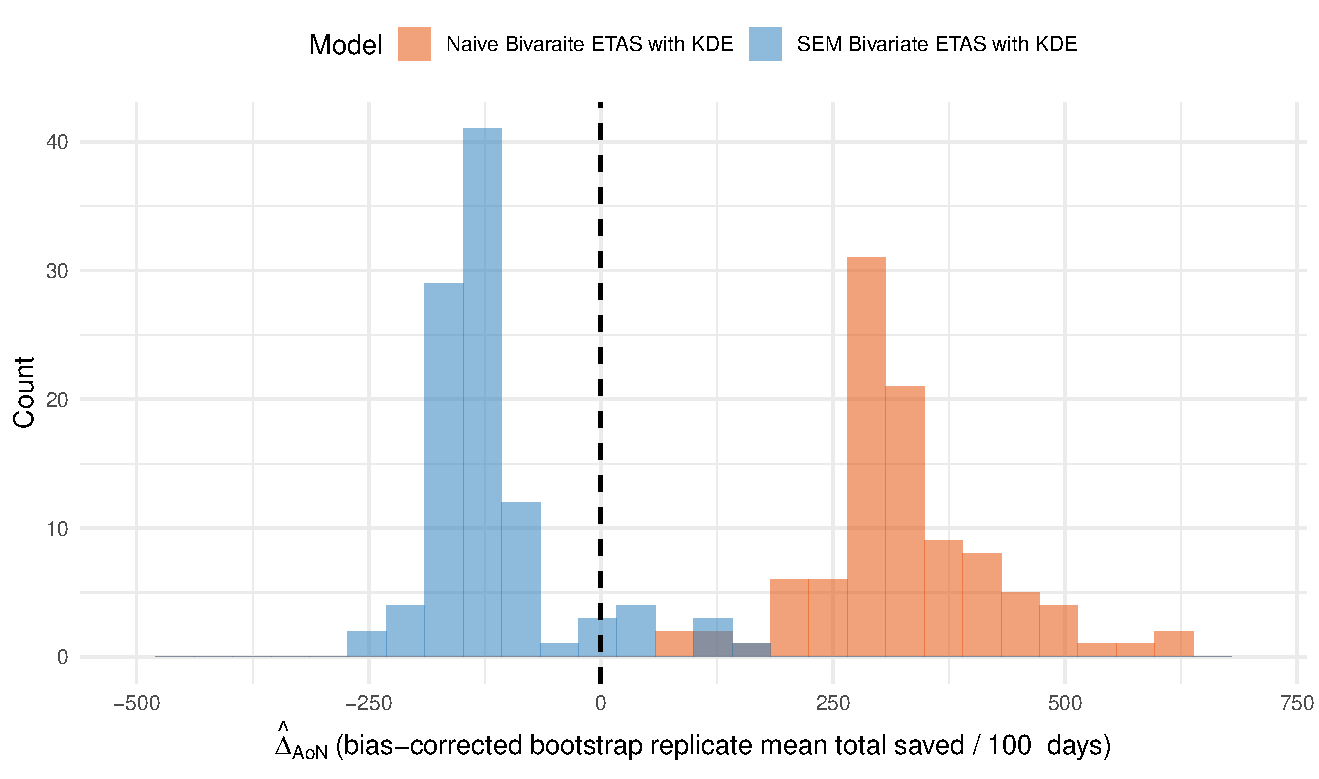
\includegraphics[width=0.8\linewidth]{plots/oklahoma/ATE_diff.pdf}
\caption{De-biased Bootstrap replicate distribution of all-or-nothing total saved for Naive vs SEM approach. The dashed vertical line marks zero savings.}
\label{fig:ok-ef-bootstrap-hist}
\end{figure}

The SEM approach materially changes the policy contrast relative to the naive counterpart. Under the same 100-day horizon, the expected saved events contrast from the SEM suggests policy ineffectiveness versus the effectiveness suggested by the naive labelling approach.

This is the opposite of our initial intuition. We expected the main feature to be carry over, rather than spillover, which is true. However, we thought that the naive approach would thus over estimate the productivity of the treatment process, and suggest that the treatment had not decreased the productivity. In fact the flexibility of the model, with full self excitation appears able to account for this, and under the label misspecification suggests that the treatment did indeed save some earthquakes. However, we note that under the SEM were points are plausibly relabelled to their true process, the same flexibility specification suggests there is little to no saving of earthquakes. When observing the cumulative count of earthquakes Figure \ref{fig:cumulative_count} this appears reasonable with the observation that earthquakes did not decrease immediately after the directive went in to force.

\begin{figure}[htbp]
\centering
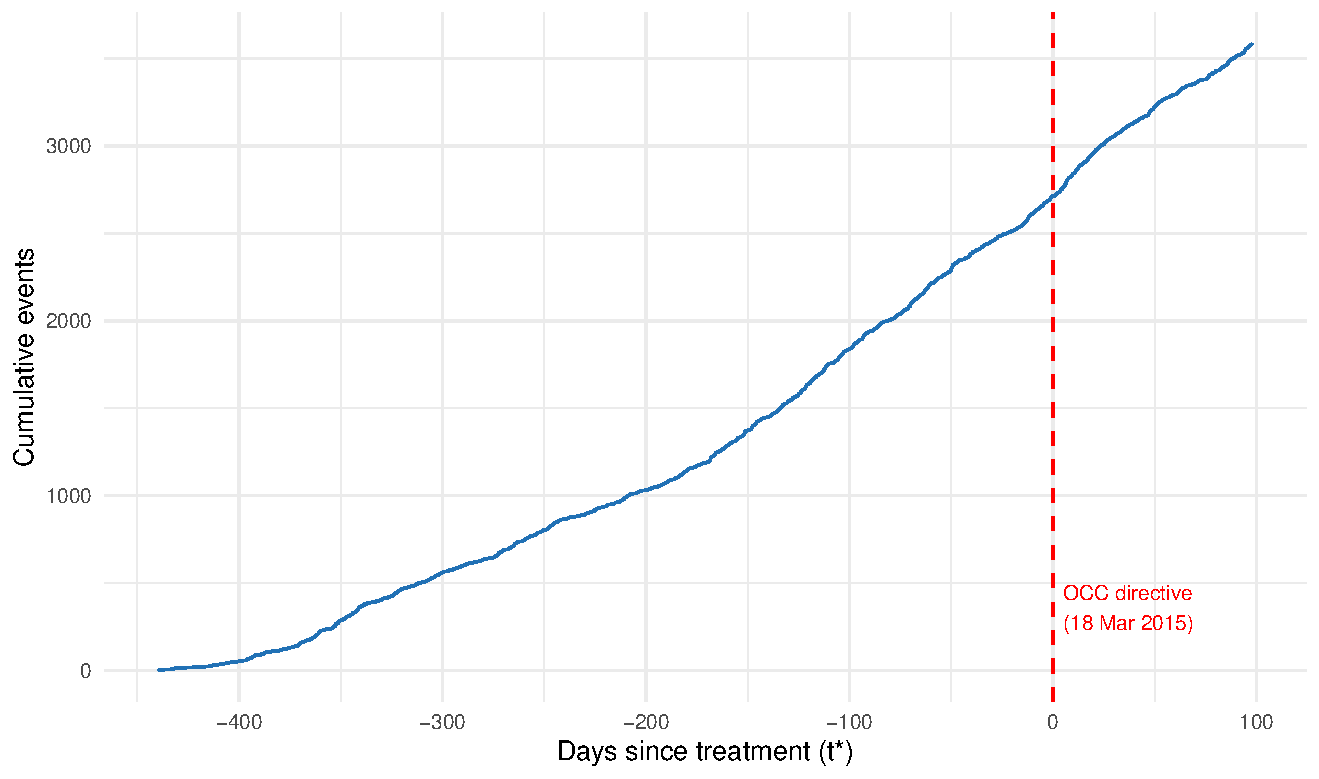
\includegraphics[width=0.85\linewidth]{plots/oklahoma/cumulative_count.pdf}
\caption{Cumulative counts of earthquakes in Oklahoma with magnitude at least 2.5 (regional catalog at or above the analysis threshold $m_0$). Vertical line: OCC directive at $t^*$.}
\label{fig:cumulative_count}
\end{figure}

Aside from our analysis, there are scientific reasons why the treatment should decrease seismicity \cite{LangenbruchZoback2016,Hincks2018}. Our approach suggests that one must wait longer before drawing such conclusions, particularly in an area where spillover and carry over are long range, so the effects of the control process pre treatment, or outside the treatment area cannot be safely disregarded.

% Optional (bootstrap moment summary; see Appendix~\ref{app:oklahoma}):
% \input{inst/oklahoma/paper/generated/tab_ok_bootstrap_summary}

% Preamble: \usepackage{booktabs}

\section{Seismic Activity in Oklahoma}\label{sec:application}

A sharp rise in seismicity in the US state of Oklahoma was observed after 2008. Existing research \cite{Keranen2014,WeingartenEtAl2015} attributes this increase primarily to high-volume wastewater (produced-water) disposal, especially disposal into the deep Arbuckle rock formations near basement-connected faults, rather than to hydraulic fracturing. Subsequent analyses \citep{WalshZoback2015} showed that earthquake activity clustered near large volume disposal wells and closely tracked rapid increases in disposal volumes in central Oklahoma . Later work refined the mechanism, emphasizing injection depth relative to crystalline basement and delayed pressure diffusion, which help explain both the regional spread of seismicity and the lagged decline in earthquake rates after disposal volumes were reduced \cite{LangenbruchZoback2016,Hincks2018}. Although Oklahoma has also experienced earthquakes directly associated with hydraulic-fracturing stages, that literature generally treats them as a distinct process and a smaller contributor to the statewide surge in seismicity during the 2010s \cite{RubinsteinMahani2015,SkoumalEtAl2018}.

On 18 March 2015 the Oklahoma Corporation Commission (OCC) issued a directive requiring disposal well operators within a designated Area of Interest (AOI) in central Oklahoma to reduce wastewater disposal volumes \cite{wertz2015regulators}. The AOI is a seismicly active area, where the Arbuckle rock formation is well suited to absorbing liquid. While a decline in seismicity is readily observed after the directive, estimating the actual causal effect of the policy is challenging due to temporal carry over, spatial spillover and non random treatment assignment. We target a DTAITE estimate where the comparison is control everywhere in Oklahoma vs the actual treatment regime, thus we will estimate the expected number of Earthquakes the policy prevented.

We restrict to earthquakes of at least magnitude 2.5 and consider bivariate epidemic-type aftershock sequence (ETAS) models \cite{ogata} for latent control and treated components with a shared triggering kernel and KDE-driven inhomogeneous background \cite{nandan2017objective}. We use the fist half of the pre treatment data to estimate the background rate and proceed with our SEM approach comparing it to the naive approach setting labels equal to the location treatment status.

Our chosen estimand of interest is the 100 day DTAITE, where the two treatment regimes are control everywhere, i.e. no directive was made and the actual observed treatment regime, denoted $\hat\Delta_{\mathrm{AoI}}=E[N(\mathrm{control\ everywhere})]-E[N(\mathrm{actual\ regime})]$. Table \ref{tab:ok_counts} shows the differences in expected counts for the ETAS model with parameters estimated with naive labelling and our SEM method.

% Auto-generated by oklahoma_paper_assets.R — do not edit by hand
\begin{table}
\caption{\label{tab:ok_counts}Observed and model-implied all-or-nothing expected counts naive and SEM approach.}
\centering
\begin{tabular}[t]{lrrr}
\toprule
Method & $E[N_C]$ & $E[N_A]$ & $\Delta=E[N_C]-E[N_A]$\\
\midrule
Naive & 946 & 605 & 341\\
SEM & 334 & 453 & -118\\
\bottomrule
\end{tabular}
\end{table}


Figure \ref{fig:ok-ef-bootstrap-hist} shows the distributions of a parametric bootstrapped DTAITE estimands using de-biased bootstrap replicates \cite{efron_boot}, there is limited overlap between the distributions suggesting a real difference.

\begin{figure}[htbp]
\centering
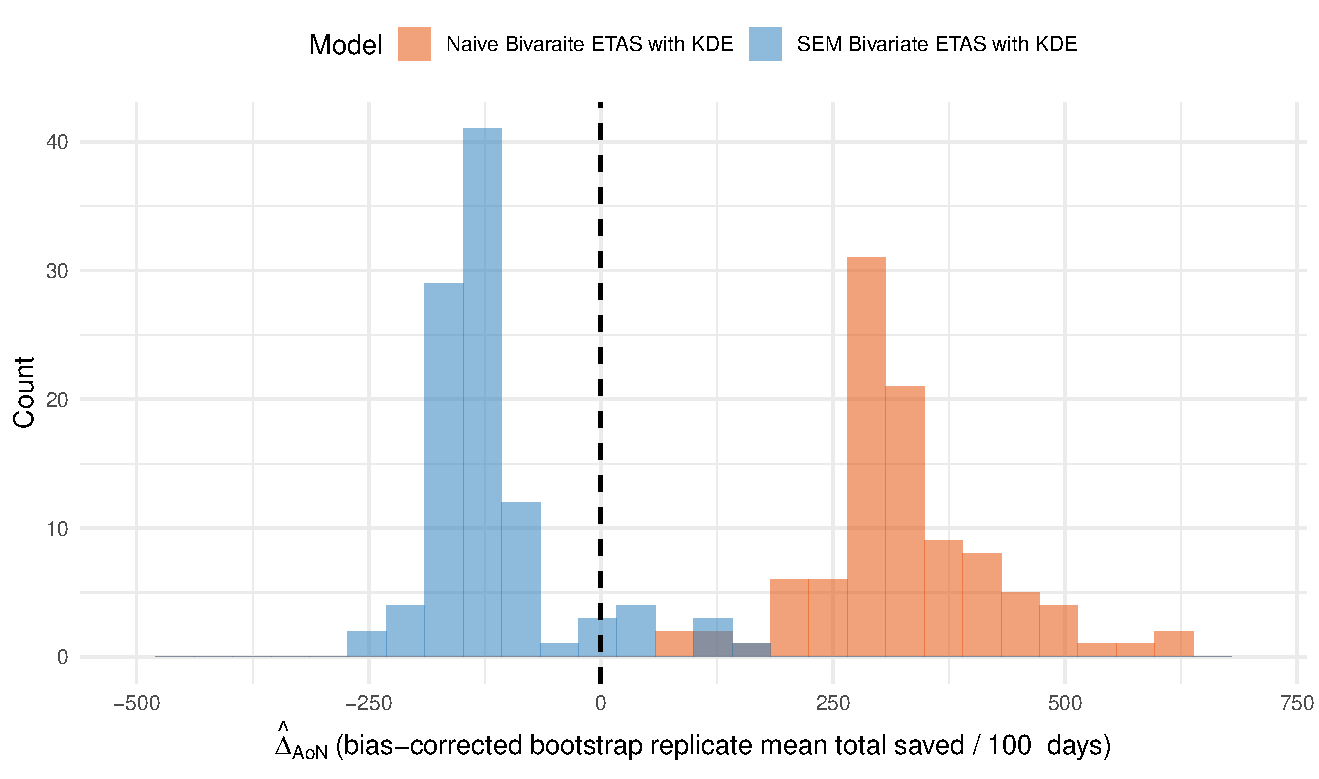
\includegraphics[width=0.8\linewidth]{plots/oklahoma/ATE_diff.pdf}
\caption{De-biased Bootstrap replicate distribution of all-or-nothing total saved for Naive vs SEM approach. The dashed vertical line marks zero savings.}
\label{fig:ok-ef-bootstrap-hist}
\end{figure}

The SEM approach materially changes the policy contrast relative to the naive counterpart. Under the same 100-day horizon, the expected saved events contrast from the SEM suggests policy ineffectiveness versus the effectiveness suggested by the naive labelling approach.

This is the opposite of our initial intuition. We expected the main feature to be carry over, rather than spillover, which is true. However, we thought that the naive approach would thus over estimate the productivity of the treatment process, and suggest that the treatment had not decreased the productivity. In fact the flexibility of the model, with full self excitation appears able to account for this, and under the label misspecification suggests that the treatment did indeed save some earthquakes. However, we note that under the SEM were points are plausibly relabelled to their true process, the same flexibility specification suggests there is little to no saving of earthquakes. When observing the cumulative count of earthquakes Figure \ref{fig:cumulative_count} this appears reasonable with the observation that earthquakes did not decrease immediately after the directive went in to force.

\begin{figure}[htbp]
\centering
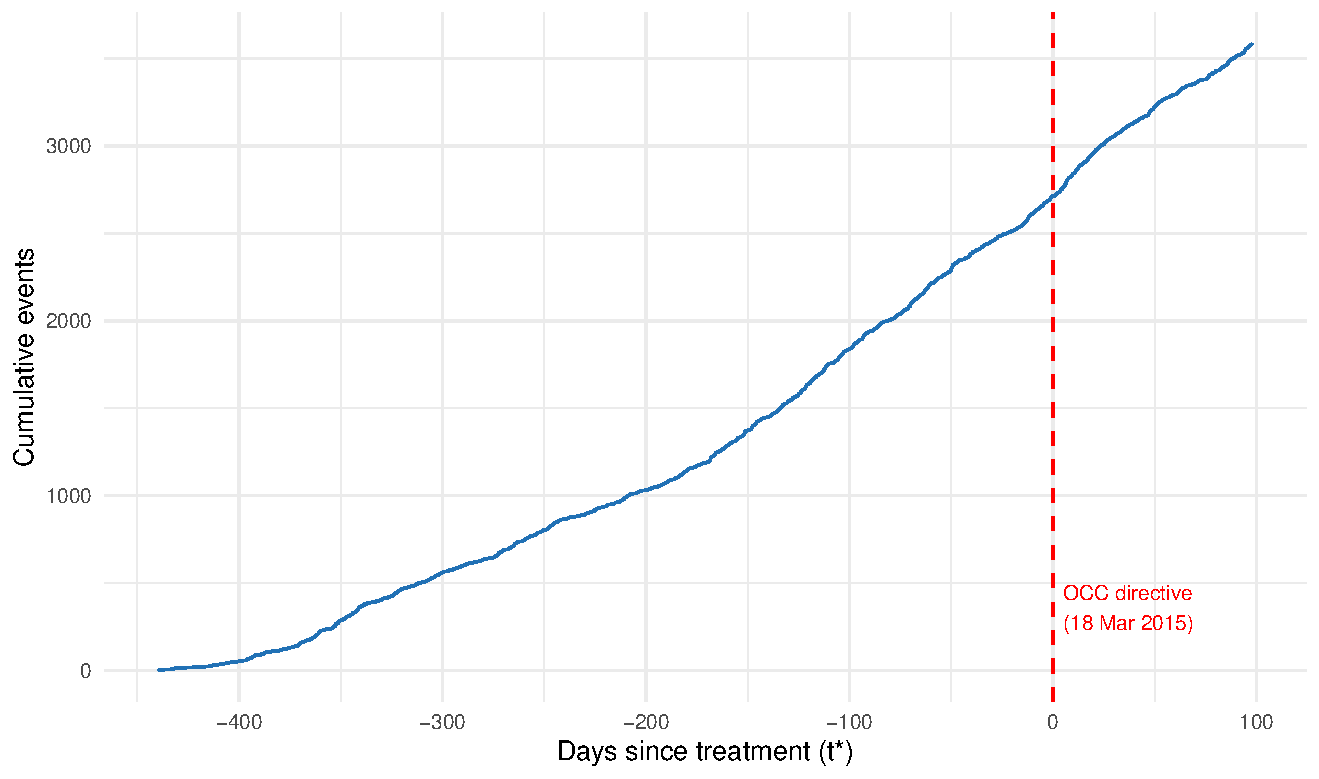
\includegraphics[width=0.85\linewidth]{plots/oklahoma/cumulative_count.pdf}
\caption{Cumulative counts of earthquakes in Oklahoma with magnitude at least 2.5 (regional catalog at or above the analysis threshold $m_0$). Vertical line: OCC directive at $t^*$.}
\label{fig:cumulative_count}
\end{figure}

Aside from our analysis, there are scientific reasons why the treatment should decrease seismicity \cite{LangenbruchZoback2016,Hincks2018}. Our approach suggests that one must wait longer before drawing such conclusions, particularly in an area where spillover and carry over are long range, so the effects of the control process pre treatment, or outside the treatment area cannot be safely disregarded.

% Optional (bootstrap moment summary; see Appendix~\ref{app:oklahoma}):
% % Auto-generated by oklahoma_paper_assets.R
\begin{table}
\caption{\label{tab:ok_bootstrap_summary}Bootstrap summary (bias-corrected replicate means of $\hat\Delta_{\mathrm{AoN}}$, days matching analysis window).}
\centering
\begin{tabular}[t]{@{}lrrrrrr@{}}
\toprule
Model & $n$ & Mean & SD & 2.5\% & 50\% & 97.5\%\\
\midrule
Naive & 100 & 340.7 & 191.7 & 115.3 & 308.1 & 588.6\\
SEM & 100 & -118.4 & 74.0 & -210.0 & -139.2 & 119.3\\
\bottomrule
\end{tabular}
\end{table}


% Preamble: \usepackage{booktabs}

\section{Seismic Activity in Oklahoma}\label{sec:application}

A sharp rise in seismicity in the US state of Oklahoma was observed after 2008. Existing research \cite{Keranen2014,WeingartenEtAl2015} attributes this increase primarily to high-volume wastewater (produced-water) disposal, especially disposal into the deep Arbuckle rock formations near basement-connected faults, rather than to hydraulic fracturing. Subsequent analyses \citep{WalshZoback2015} showed that earthquake activity clustered near large volume disposal wells and closely tracked rapid increases in disposal volumes in central Oklahoma . Later work refined the mechanism, emphasizing injection depth relative to crystalline basement and delayed pressure diffusion, which help explain both the regional spread of seismicity and the lagged decline in earthquake rates after disposal volumes were reduced \cite{LangenbruchZoback2016,Hincks2018}. Although Oklahoma has also experienced earthquakes directly associated with hydraulic-fracturing stages, that literature generally treats them as a distinct process and a smaller contributor to the statewide surge in seismicity during the 2010s \cite{RubinsteinMahani2015,SkoumalEtAl2018}.

On 18 March 2015 the Oklahoma Corporation Commission (OCC) issued a directive requiring disposal well operators within a designated Area of Interest (AOI) in central Oklahoma to reduce wastewater disposal volumes \cite{wertz2015regulators}. The AOI is a seismicly active area, where the Arbuckle rock formation is well suited to absorbing liquid. While a decline in seismicity is readily observed after the directive, estimating the actual causal effect of the policy is challenging due to temporal carry over, spatial spillover and non random treatment assignment. We target a DTAITE estimate where the comparison is control everywhere in Oklahoma vs the actual treatment regime, thus we will estimate the expected number of Earthquakes the policy prevented.

We restrict to earthquakes of at least magnitude 2.5 and consider bivariate epidemic-type aftershock sequence (ETAS) models \cite{ogata} for latent control and treated components with a shared triggering kernel and KDE-driven inhomogeneous background \cite{nandan2017objective}. We use the fist half of the pre treatment data to estimate the background rate and proceed with our SEM approach comparing it to the naive approach setting labels equal to the location treatment status.

Our chosen estimand of interest is the 100 day DTAITE, where the two treatment regimes are control everywhere, i.e. no directive was made and the actual observed treatment regime, denoted $\hat\Delta_{\mathrm{AoI}}=E[N(\mathrm{control\ everywhere})]-E[N(\mathrm{actual\ regime})]$. Table \ref{tab:ok_counts} shows the differences in expected counts for the ETAS model with parameters estimated with naive labelling and our SEM method.

% Auto-generated by oklahoma_paper_assets.R — do not edit by hand
\begin{table}
\caption{\label{tab:ok_counts}Observed and model-implied all-or-nothing expected counts naive and SEM approach.}
\centering
\begin{tabular}[t]{lrrr}
\toprule
Method & $E[N_C]$ & $E[N_A]$ & $\Delta=E[N_C]-E[N_A]$\\
\midrule
Naive & 946 & 605 & 341\\
SEM & 334 & 453 & -118\\
\bottomrule
\end{tabular}
\end{table}


Figure \ref{fig:ok-ef-bootstrap-hist} shows the distributions of a parametric bootstrapped DTAITE estimands using de-biased bootstrap replicates \cite{efron_boot}, there is limited overlap between the distributions suggesting a real difference.

\begin{figure}[htbp]
\centering
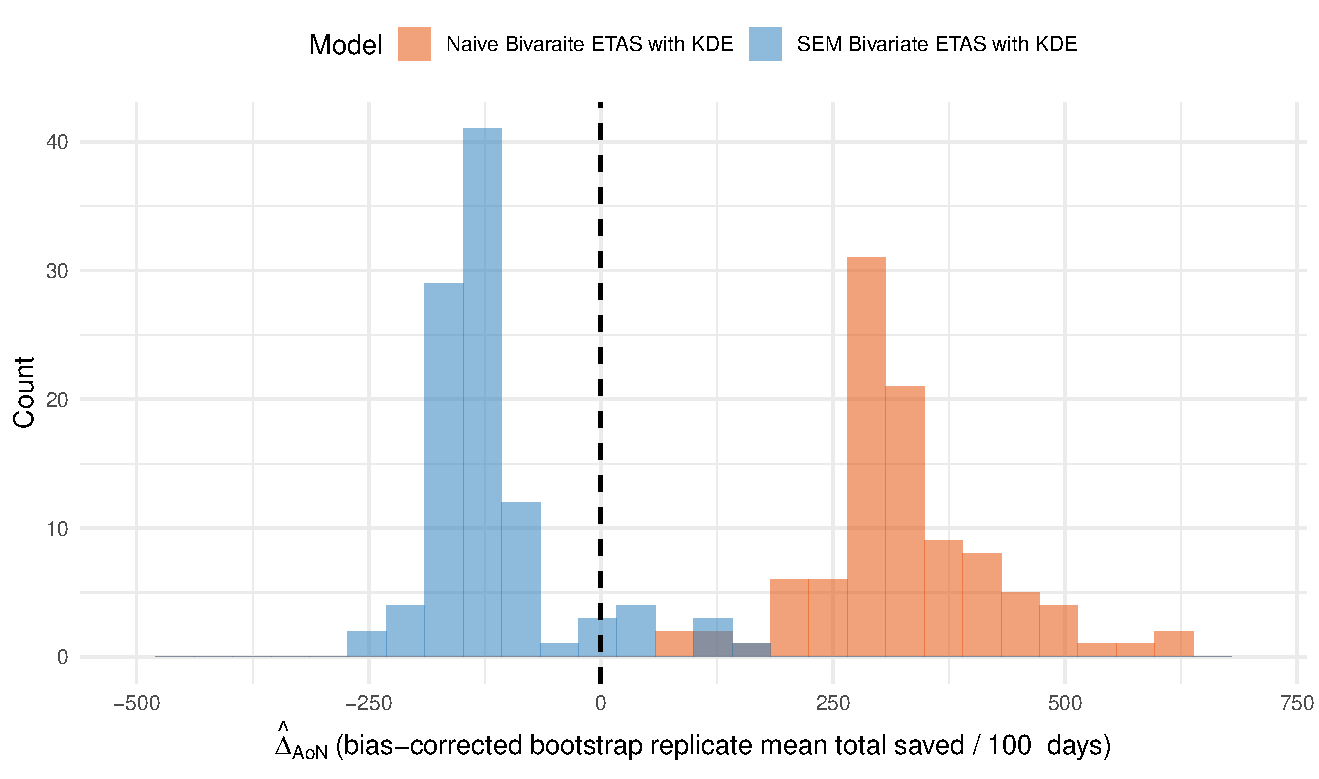
\includegraphics[width=0.8\linewidth]{plots/oklahoma/ATE_diff.pdf}
\caption{De-biased Bootstrap replicate distribution of all-or-nothing total saved for Naive vs SEM approach. The dashed vertical line marks zero savings.}
\label{fig:ok-ef-bootstrap-hist}
\end{figure}

The SEM approach materially changes the policy contrast relative to the naive counterpart. Under the same 100-day horizon, the expected saved events contrast from the SEM suggests policy ineffectiveness versus the effectiveness suggested by the naive labelling approach.

This is the opposite of our initial intuition. We expected the main feature to be carry over, rather than spillover, which is true. However, we thought that the naive approach would thus over estimate the productivity of the treatment process, and suggest that the treatment had not decreased the productivity. In fact the flexibility of the model, with full self excitation appears able to account for this, and under the label misspecification suggests that the treatment did indeed save some earthquakes. However, we note that under the SEM were points are plausibly relabelled to their true process, the same flexibility specification suggests there is little to no saving of earthquakes. When observing the cumulative count of earthquakes Figure \ref{fig:cumulative_count} this appears reasonable with the observation that earthquakes did not decrease immediately after the directive went in to force.

\begin{figure}[htbp]
\centering
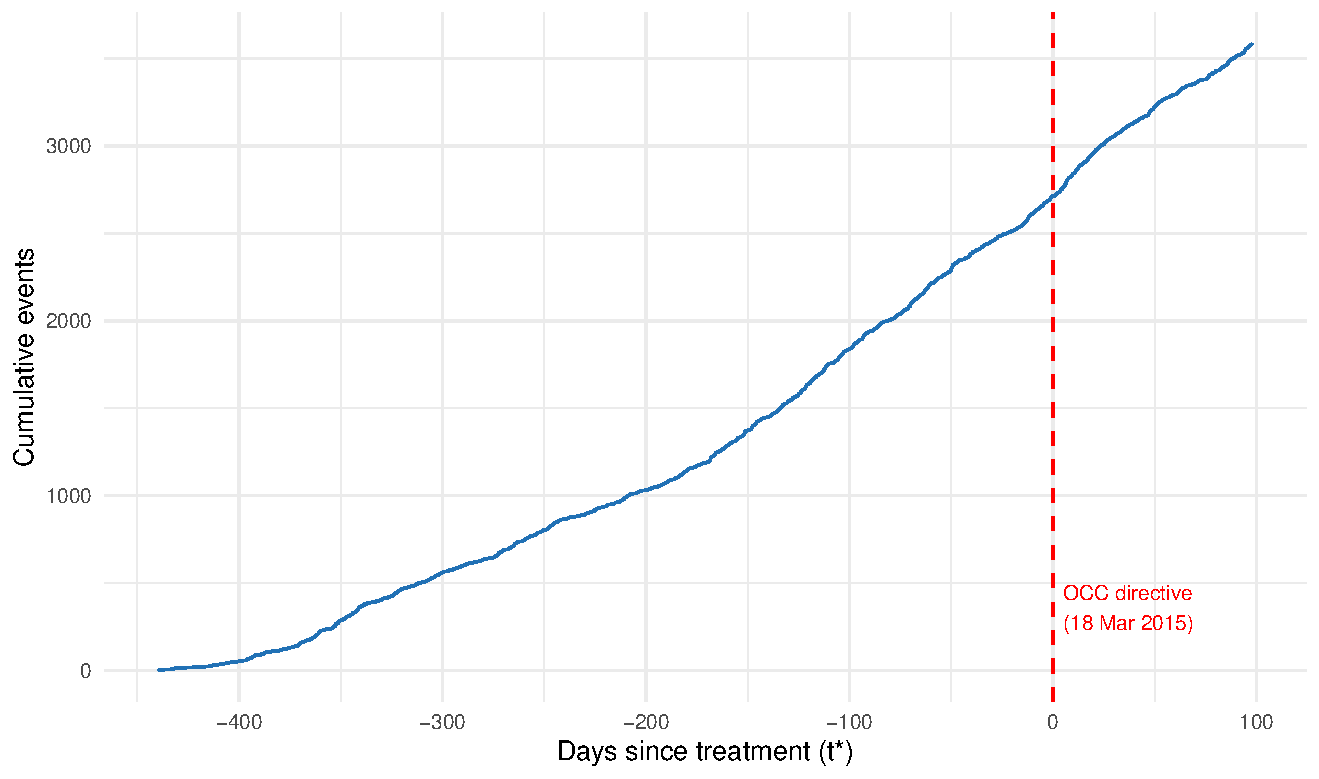
\includegraphics[width=0.85\linewidth]{plots/oklahoma/cumulative_count.pdf}
\caption{Cumulative counts of earthquakes in Oklahoma with magnitude at least 2.5 (regional catalog at or above the analysis threshold $m_0$). Vertical line: OCC directive at $t^*$.}
\label{fig:cumulative_count}
\end{figure}

Aside from our analysis, there are scientific reasons why the treatment should decrease seismicity \cite{LangenbruchZoback2016,Hincks2018}. Our approach suggests that one must wait longer before drawing such conclusions, particularly in an area where spillover and carry over are long range, so the effects of the control process pre treatment, or outside the treatment area cannot be safely disregarded.

% Optional (bootstrap moment summary; see Appendix~\ref{app:oklahoma}):
% % Auto-generated by oklahoma_paper_assets.R
\begin{table}
\caption{\label{tab:ok_bootstrap_summary}Bootstrap summary (bias-corrected replicate means of $\hat\Delta_{\mathrm{AoN}}$, days matching analysis window).}
\centering
\begin{tabular}[t]{@{}lrrrrrr@{}}
\toprule
Model & $n$ & Mean & SD & 2.5\% & 50\% & 97.5\%\\
\midrule
Naive & 100 & 340.7 & 191.7 & 115.3 & 308.1 & 588.6\\
SEM & 100 & -118.4 & 74.0 & -210.0 & -139.2 & 119.3\\
\bottomrule
\end{tabular}
\end{table}


% Preamble: \usepackage{booktabs}

\section{Seismic Activity in Oklahoma}\label{sec:application}

A sharp rise in seismicity in the US state of Oklahoma was observed after 2008. Existing research \cite{Keranen2014,WeingartenEtAl2015} attributes this increase primarily to high-volume wastewater (produced-water) disposal, especially disposal into the deep Arbuckle rock formations near basement-connected faults, rather than to hydraulic fracturing. Subsequent analyses \citep{WalshZoback2015} showed that earthquake activity clustered near large volume disposal wells and closely tracked rapid increases in disposal volumes in central Oklahoma . Later work refined the mechanism, emphasizing injection depth relative to crystalline basement and delayed pressure diffusion, which help explain both the regional spread of seismicity and the lagged decline in earthquake rates after disposal volumes were reduced \cite{LangenbruchZoback2016,Hincks2018}. Although Oklahoma has also experienced earthquakes directly associated with hydraulic-fracturing stages, that literature generally treats them as a distinct process and a smaller contributor to the statewide surge in seismicity during the 2010s \cite{RubinsteinMahani2015,SkoumalEtAl2018}.

On 18 March 2015 the Oklahoma Corporation Commission (OCC) issued a directive requiring disposal well operators within a designated Area of Interest (AOI) in central Oklahoma to reduce wastewater disposal volumes \cite{wertz2015regulators}. The AOI is a seismicly active area, where the Arbuckle rock formation is well suited to absorbing liquid. While a decline in seismicity is readily observed after the directive, estimating the actual causal effect of the policy is challenging due to temporal carry over, spatial spillover and non random treatment assignment. We target a DTAITE estimate where the comparison is control everywhere in Oklahoma vs the actual treatment regime, thus we will estimate the expected number of Earthquakes the policy prevented.

We restrict to earthquakes of at least magnitude 2.5 and consider bivariate epidemic-type aftershock sequence (ETAS) models \cite{ogata} for latent control and treated components with a shared triggering kernel and KDE-driven inhomogeneous background \cite{nandan2017objective}. We use the fist half of the pre treatment data to estimate the background rate and proceed with our SEM approach comparing it to the naive approach setting labels equal to the location treatment status.

Our chosen estimand of interest is the 100 day DTAITE, where the two treatment regimes are control everywhere, i.e. no directive was made and the actual observed treatment regime, denoted $\hat\Delta_{\mathrm{AoI}}=E[N(\mathrm{control\ everywhere})]-E[N(\mathrm{actual\ regime})]$. Table \ref{tab:ok_counts} shows the differences in expected counts for the ETAS model with parameters estimated with naive labelling and our SEM method.

% Auto-generated by oklahoma_paper_assets.R — do not edit by hand
\begin{table}
\caption{\label{tab:ok_counts}Observed and model-implied all-or-nothing expected counts naive and SEM approach.}
\centering
\begin{tabular}[t]{lrrr}
\toprule
Method & $E[N_C]$ & $E[N_A]$ & $\Delta=E[N_C]-E[N_A]$\\
\midrule
Naive & 946 & 605 & 341\\
SEM & 334 & 453 & -118\\
\bottomrule
\end{tabular}
\end{table}


Figure \ref{fig:ok-ef-bootstrap-hist} shows the distributions of a parametric bootstrapped DTAITE estimands using de-biased bootstrap replicates \cite{efron_boot}, there is limited overlap between the distributions suggesting a real difference.

\begin{figure}[htbp]
\centering
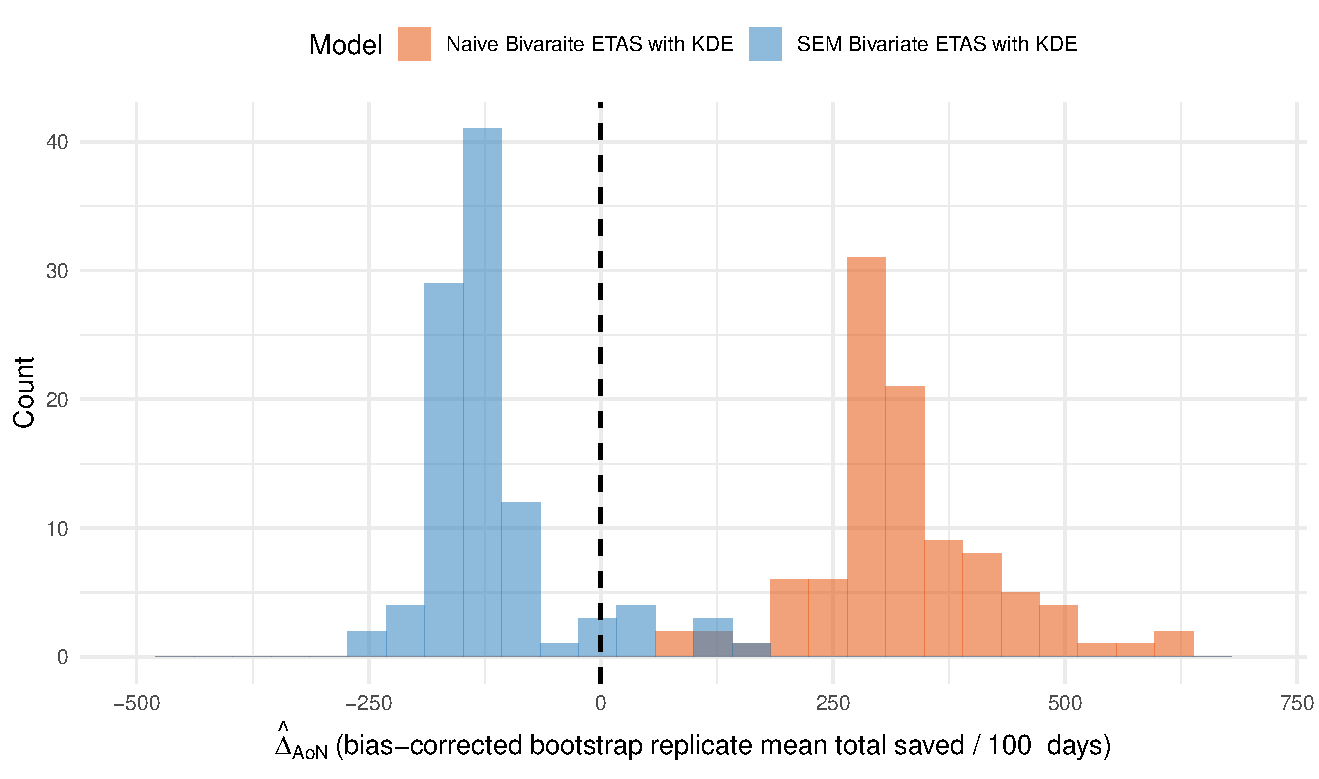
\includegraphics[width=0.8\linewidth]{plots/oklahoma/ATE_diff.pdf}
\caption{De-biased Bootstrap replicate distribution of all-or-nothing total saved for Naive vs SEM approach. The dashed vertical line marks zero savings.}
\label{fig:ok-ef-bootstrap-hist}
\end{figure}

The SEM approach materially changes the policy contrast relative to the naive counterpart. Under the same 100-day horizon, the expected saved events contrast from the SEM suggests policy ineffectiveness versus the effectiveness suggested by the naive labelling approach.

This is the opposite of our initial intuition. We expected the main feature to be carry over, rather than spillover, which is true. However, we thought that the naive approach would thus over estimate the productivity of the treatment process, and suggest that the treatment had not decreased the productivity. In fact the flexibility of the model, with full self excitation appears able to account for this, and under the label misspecification suggests that the treatment did indeed save some earthquakes. However, we note that under the SEM were points are plausibly relabelled to their true process, the same flexibility specification suggests there is little to no saving of earthquakes. When observing the cumulative count of earthquakes Figure \ref{fig:cumulative_count} this appears reasonable with the observation that earthquakes did not decrease immediately after the directive went in to force.

\begin{figure}[htbp]
\centering
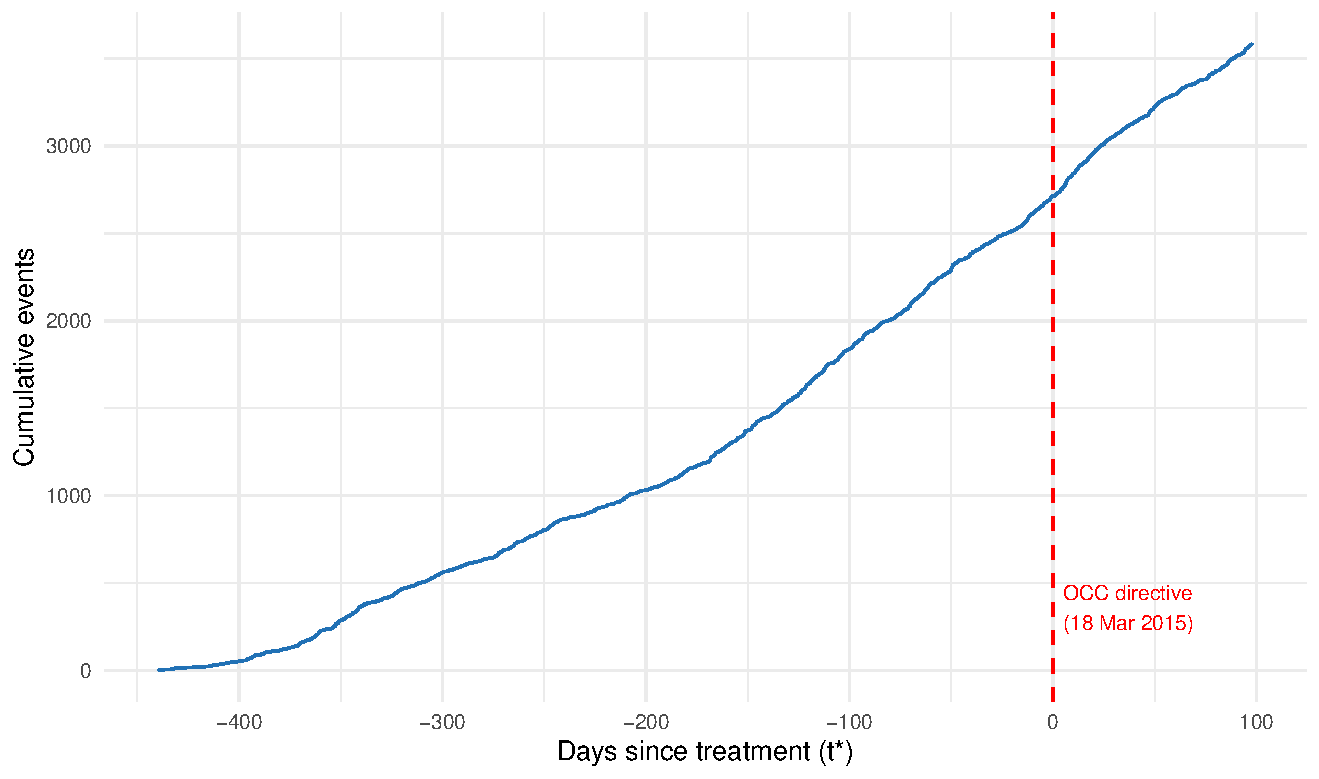
\includegraphics[width=0.85\linewidth]{plots/oklahoma/cumulative_count.pdf}
\caption{Cumulative counts of earthquakes in Oklahoma with magnitude at least 2.5 (regional catalog at or above the analysis threshold $m_0$). Vertical line: OCC directive at $t^*$.}
\label{fig:cumulative_count}
\end{figure}

Aside from our analysis, there are scientific reasons why the treatment should decrease seismicity \cite{LangenbruchZoback2016,Hincks2018}. Our approach suggests that one must wait longer before drawing such conclusions, particularly in an area where spillover and carry over are long range, so the effects of the control process pre treatment, or outside the treatment area cannot be safely disregarded.

% Optional (bootstrap moment summary; see Appendix~\ref{app:oklahoma}):
% % Auto-generated by oklahoma_paper_assets.R
\begin{table}
\caption{\label{tab:ok_bootstrap_summary}Bootstrap summary (bias-corrected replicate means of $\hat\Delta_{\mathrm{AoN}}$, days matching analysis window).}
\centering
\begin{tabular}[t]{@{}lrrrrrr@{}}
\toprule
Model & $n$ & Mean & SD & 2.5\% & 50\% & 97.5\%\\
\midrule
Naive & 100 & 340.7 & 191.7 & 115.3 & 308.1 & 588.6\\
SEM & 100 & -118.4 & 74.0 & -210.0 & -139.2 & 119.3\\
\bottomrule
\end{tabular}
\end{table}

